%%%%%%%%%%%%%%%%%%%%%%%%%%%%%%%%%%%%%%%%%%%%%%%%%%%%%%%%%%%%%%%%%%%%%%%%%%%
%
% Template for a LaTex article in English.
%
%%%%%%%%%%%%%%%%%%%%%%%%%%%%%%%%%%%%%%%%%%%%%%%%%%%%%%%%%%%%%%%%%%%%%%%%%%%

\documentclass{article}

% AMS packages:
\usepackage{amsmath, amsthm, amsfonts}
\usepackage{graphicx}

% Theorems
%-----------------------------------------------------------------
\newtheorem{thm}{Theorem}[section]
\newtheorem{cor}[thm]{Corollary}
\newtheorem{lem}[thm]{Lemma}
\newtheorem{prop}[thm]{Proposition}
\theoremstyle{definition}
\newtheorem{defn}[thm]{Definition}
\theoremstyle{remark}
\newtheorem{rem}[thm]{Remark}

% Shortcuts.
% One can define new commands to shorten frequently used
% constructions. As an example, this defines the R and Z used
% for the real and integer numbers.
%-----------------------------------------------------------------
\def\RR{\mathbb{R}}
\def\ZZ{\mathbb{Z}}

% Similarly, one can define commands that take arguments. In this
% example we define a command for the absolute value.
% -----------------------------------------------------------------
\newcommand{\abs}[1]{\left\vert#1\right\vert}

% Operators
% New operators must defined as such to have them typeset
% correctly. As an example we define the Jacobian:
% -----------------------------------------------------------------
\DeclareMathOperator{\Jac}{Jac}

%-----------------------------------------------------------------
\title{Variability in Feed Forward Neural Network}
\author{NIVHSA\\
  \small India}

\begin{document}
\maketitle

\abstract{Weights of a simple Feed Forward Neural Network (FFNN) attain finite values upon first order optimisation algorithms. We propose an alternate method in which the weights are modelled as a composite function; 1) mapping between input and output spaces, optimised via back propagation algorithm 2) Information captured inherently present in the input space via clustering.}
 
\section{Introduction}
Fig.\ref{fig:NN}  illustrates a basic FFNN \cite{ffnn}, \textbf{x} is a 2-dimensional vector($x_1,x_2$) provided as two inputs to the network. 

\begin{figure}
  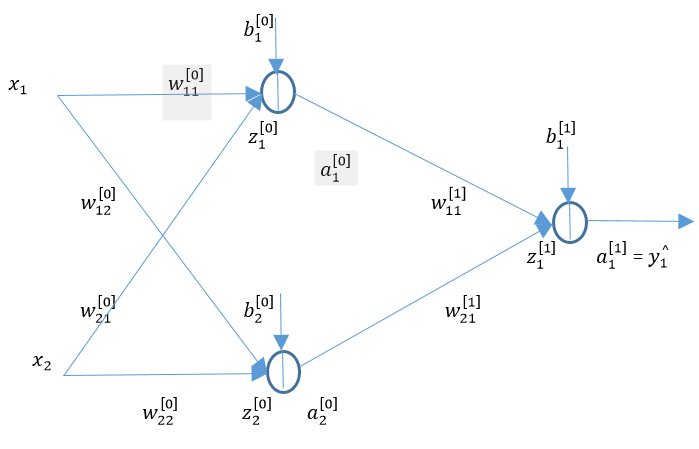
\includegraphics[width=\linewidth]{document.png}
  \caption{Feed Forward Neural network with one hidden layer}
  \label{fig:NN}
\end{figure}

The forward propagation eqs. as follows:

\begin{equation}\label{eq:fw1}
z_1^{[0]} = w_{11}^{[0]}.x_1+w_{21}^{[0]}.x_2 + b_1^{[0]};  \quad  a_1^{[0]} = \sigma(z_1^{[0]})
\end{equation}

\begin{equation}\label{eq:fw1}
z_2^{[0]} = w_{12}^{[0]}.x_1+w_{22}^{[0]}.x_2 + b_2^{[0]} ; \quad  a_2^{[0]} = \sigma(z_2^{[0]})
\end{equation}

\begin{equation}\label{eq:fw3}
z_1^{[1]} = w_{11}^{[1]}.a_1^{[0]}+w_{21}^{[1]}.a_2^{[0]} + b_1^{[1]} ; \quad  a_1^{[1]} = \sigma(z_1^{[1]})
\end{equation}
where $\sigma$ is the sigmoid function. 

The Backward Propagation eqs. as follows:
\begin{equation}\label{eq:bp1}
l = \hat{y_1} - y_1
\end{equation}
We consider stochastic gradient descent (SGD) algorithm \cite{sgd}.
\begin{equation}
 w_{ij} := w_{ij}-\alpha.\frac{\partial l}{\partial w_{ij}}, 
 \label{eq:wt}
\end{equation}

where $\alpha$ is the learning rate. 
For e.g., from Fig.\ref{fig:NN} $$ w_{21}^{[0]}:= w_{21}^{[0]} -\alpha.\frac{\partial l}{\partial w_{21}^{[0]}}$$
Where $$ \frac{\partial l}{\partial w_{21}^{[0]}} = \frac{\partial l}{\partial a_{1}^{[1]}}.\frac{\partial a_1^{[1]}}{\partial z_1^{[1]}}.
\frac{\partial z_1^{[1]}}{\partial a_1^{[0]}}.\frac{\partial a_1^{[0]}}{\partial z_1^{[0]}}.\frac{\partial z_1^{[0]}}{\partial w_{21}^{[0]}}$$

\section{Methods}
The weight $$w_{ij} = \frac{1}{\sqrt{2.\pi}.\sigma_{ij}}.e^{-{\mu_{ij}^2}/(2.\sigma_{ij}^2)}$$ and the weight update equation upon modification  from eq.\ref{eq:wt}, we get 
$$
k.e^{-{\mu_{ij}^2}/(2.\sigma_{ij}^2)}:= k.e^{-{\mu_{ij}^2}/(2.\sigma_{ij}^2)}-\alpha.\frac{\partial l}{\partial \mu_{ij}}.\frac{d\mu_{ij}}{dw_{ij}}; \quad  k = \frac{1}{\sqrt{2.\pi}.\sigma_{ij}}
$$
Now, $d\mu_{ij}/dw_{ij} = [dw_{ij}/d\mu_{ij}]^{-1} = -\frac{\sigma_{ij}}{k.\mu_{ij}}.e^{-{\mu_{ij}^2}/(2.\sigma_{ij}^2)}$
$$
k.e^{-{\mu_{ij}^2}/(2.\sigma_{ij}^2)}:=k.e^{-{\mu_{ij}^2}/(2.\sigma_{ij}^2)}+\alpha.\frac{\sigma_{ij}^2}{k.\mu_{ij}}.e^{{\mu_{ij}^2}/(2.\sigma_{ij}^2)}.\frac{\partial l}{\partial \mu_{ij}}
$$
The final new weight update equation is given by:
\begin{equation}
\mu_{ij} := \mu_{ij} + \alpha.\frac{\sigma_{ij}^2}{k^2}.e^{{\mu_{ij}^2}/(\sigma_{ij}^2)}.\frac{\partial l}{\partial \mu_{ij}}
\label{eq:newwteq}
\end{equation}

Deviation in eq. \ref{eq:newwteq},  $$\sigma_{ij} = ||\textbf{x}-\textbf{x}_c||_2$$, where $\textbf{x}_c$ is the centroid obtained by cluster centre computed via any cluster classification algorithm such as kmeans, Gaussian Mixture Model(GMM). In the case of classification, the number of clusters equals the number of class labels while for regression based, number of clusters equals the optimal clusters computed via elbow curve or silhouette score. 



\section{Discussion}
In this paper we aimed at providing an alternative to the current back propagation algorithm in that we hope to address two factors. First, the new weight update equation is a composite function partly capturing the mapping information between the input space and output space along with information captured inherently present in the input space via clustering. Secondly, We introduced the deviation factor as a measure of variability for the weights. Intuitively, the weights are no longer finite irrespective of the inputs instead depends on the input itself, this could provide an extra degree of freedom for the weights and enhance learning. It remains to be seen via simulations as future work. 




% Bibliography
%-----------------------------------------------------------------
\begin{thebibliography}{99}


\bibitem{ffnn} Andina, Diego, Pham, D.,  Vega-Corona, Antonio,  Seijas, Juan , Torres-Garc�a, J. (2007). Neural Networks Historical Review. 
\bibitem{sgd} Rumelhart, D., Hinton, G.,  Williams, R. Learning representations by back-propagating errors. Nature 323, 533?536 (1986). https://doi.org/10.1038/323533a0


\end{thebibliography}

\end{document}
